\subsection{Osservazioni}
Osserviamo il risultato su un'immagine scelta casualmente del set creato e sulle due immagini aggiuntive.
%! l'elemento principale e' il rumore + mettere confronti

Ricordiamo che più è alto il valore del PSNR maggiore sarà la vicinanza dell'immagine corrotta rispetto alla versione originale. 

\subsubsection{Analisi immagine geometrica}
Analizziamo l'immagine img8.png al variare del valore $\sigma$:

\begin{figure}[H]
    \centering
    \begin{subfigure}{0.6\textwidth}
        \centering
        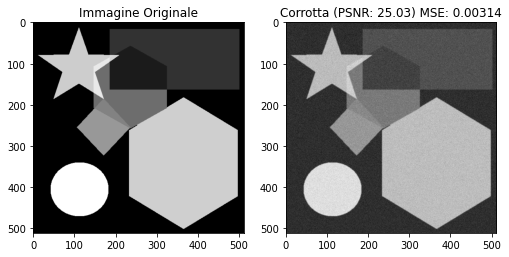
\includegraphics[width=\textwidth]{imgRel/img8corrotto/img8corrotta5x5.png}
        \caption{Img8 corrotta con $\sigma = 0.5$ dimensione $5 \times 5$}
        \label{fig: 8corrotto5}
    \end{subfigure}
    \begin{subfigure}{0.6\textwidth}
        \centering
        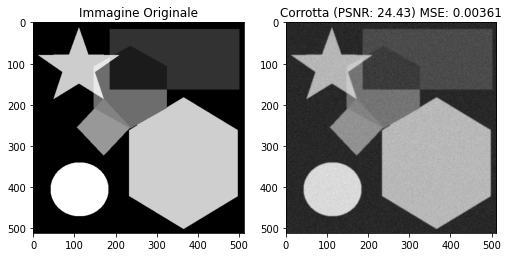
\includegraphics[width=\textwidth]{imgRel/img8corrotto/img8corrotta7x7.png}
        \caption{Img8 corrotta con $\sigma = 1$ dimensione $7\times 7$}
        \label{fig: 8corrotto7}
    \end{subfigure}
    \begin{subfigure}{0.6\textwidth}
        \centering
        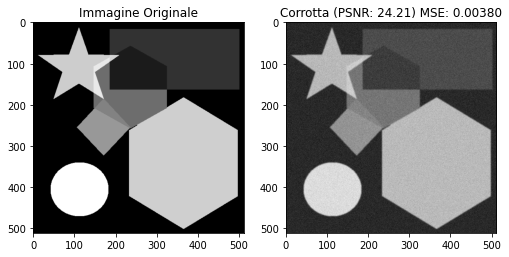
\includegraphics[width=\textwidth]{imgRel/img8corrotto/img8corrotta9x9.png}
        \caption{Img8 corrotta con $\sigma = 1.3$ dimensione $9 \times 9$}
        \label{fig: 8corrotto9}
    \end{subfigure}
    \caption{Immagine geometrica corrotta al variare di }
    \label{fig: 8corrotto}
\end{figure}
Le figure di sinistra rappresentano l'immagine originale, invece a destra sono riportate le immagini corrotte con i rispettivi valori di PSNR. 
Notiamo che all'aumentare delle dimensioni di sigma il valore di PSNR diminuisce che denota un peggioramento della qualità dell'immagine, 
infatti le immagini subiscono un'appiattimento dell'intensità della scala dei colori e i contorni delle varie figure geometriche perdono di fermezza. 
Inoltre è curioso notare.. %! da finire

\subsubsection{Analisi immagini fotografiche}
\begin{figure}[H]
    \centering
    \begin{subfigure}{0.67\textwidth}
        \centering
        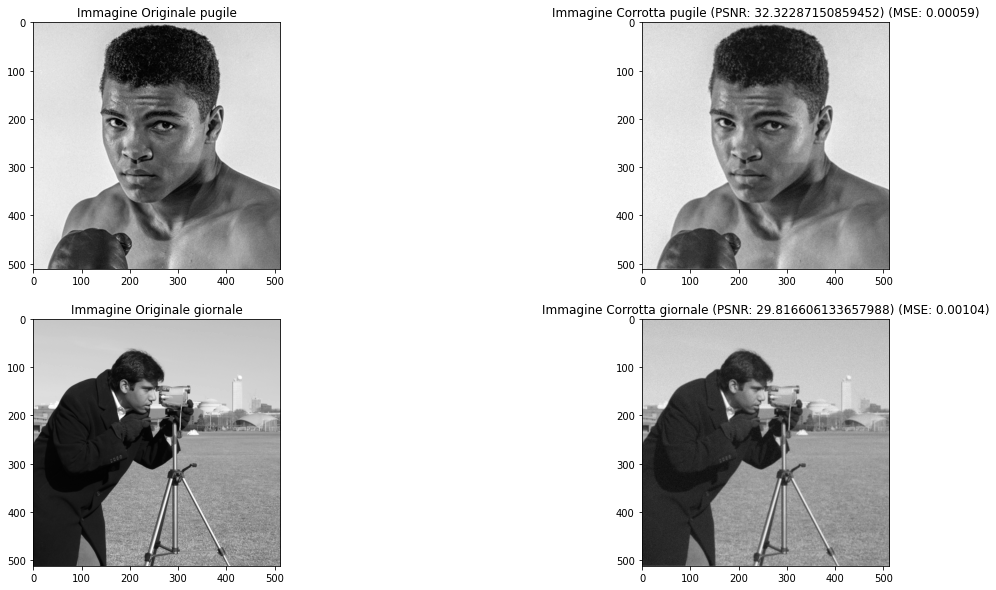
\includegraphics[width=\textwidth]{confrontiPuntoUno/5-0.5-0.02.png}
        \caption{immagini corrotte con $\sigma = 0.5$ dimensione $5 \times 5$}
        \label{fig: fotogrCorrotte5x5}
    \end{subfigure}
    \begin{subfigure}{0.67\textwidth}
        \centering
        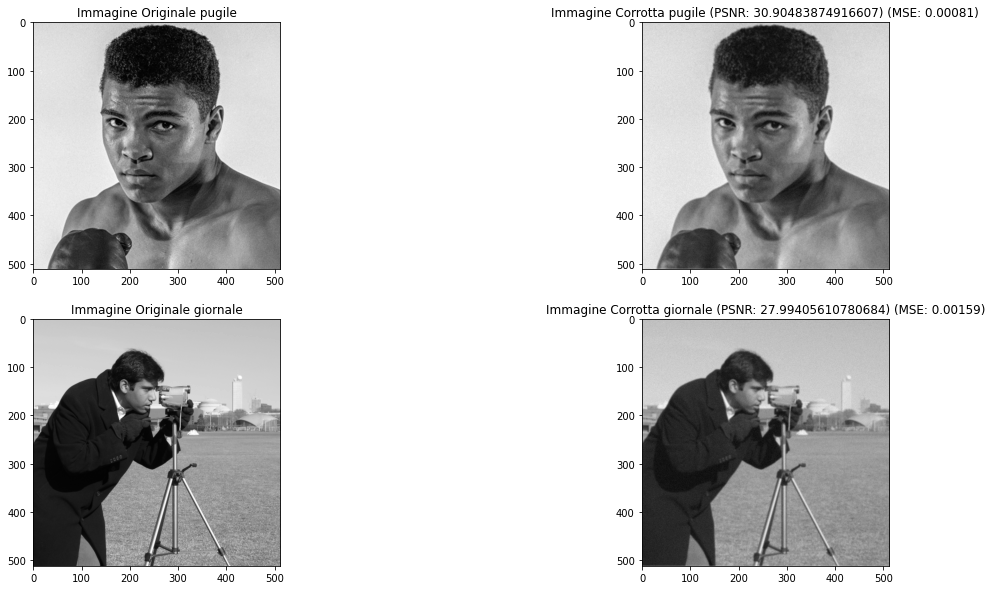
\includegraphics[width=\textwidth]{confrontiPuntoUno/7-1-0.02.png}
        \caption{immagini corrotte con $\sigma = 1$ dimensione $7 \times 7$}
        \label{fig: fotogrCorrotte7x7}
    \end{subfigure}
    \begin{subfigure}{0.67\textwidth}
        \centering
        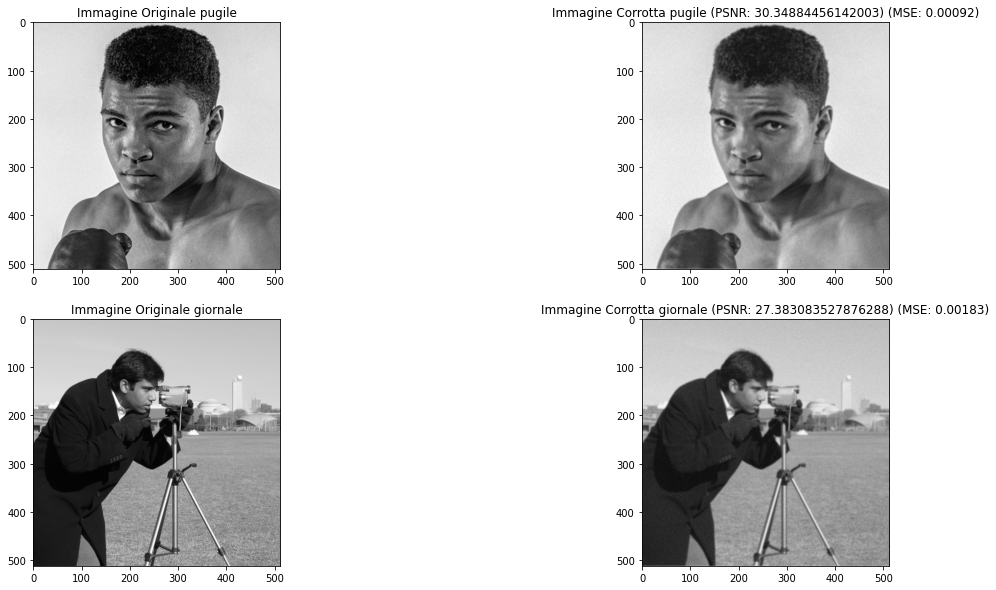
\includegraphics[width=\textwidth]{confrontiPuntoUno/9-1.3-0.02.png}
        \caption{immagini corrotte con $\sigma = 1.3$ dimensione $9 \times 9$}
        \label{fig: fotogrCorrotte9x9}
    \end{subfigure}
    \caption{Immagine fotografica corrotta al variare di $\sigma$}
    \label{fig: fotogrCorrotte}
\end{figure}
Si nota un'altra volta che all'aumentare delle dimensioni di $\sigma$ diminuisce il PSNR e l'immagine perde di 
incisività, le versioni corrotte benché risultino visivamente peggiori, si riesce ancora a ben distinguere il 
soggetto in primo piano, anche se sfocato, in tutte le immagini. 
